\documentclass{article}
\usepackage[utf8]{inputenc}
\usepackage{amsmath}
\usepackage{graphicx}
\graphicspath{ {img/} }

\title{Inteligență Artificială - Puzzle-ul lui Guarini}
\author{Ceclan Dumitru-Ioan - Sîrbu Oana-Bianca}
\date{UTCN Calculatoare, An 3, grupa 30234, 2021}

\begin{document}

\maketitle

\section{Enunțul problemei}
   
    Puzzle-ul lui Guarini este una din primele probleme inspirate din șah, formulată de Paolo Guarini in anul 1512. Problema inițială utilizează o tablă de șah de 3x3, dar pentru a putea extinde jocul pe mai multe nivele, vom folosi o tablă cu 4 rânduri si număr variabil de coloane (minim 3 coloane). 
    Inițial, pe tablă sunt plasate 6 piese de șah alcatuite doar din cai, 3 de culoare albă și 3 de culoare neagră. Caii albi se află pe primul rând al tablei, iar caii negri pe ultimul rând. 
    
    Scopul puzzle-ului este de a inversa cele două rânduri de cai.
    \begin{figure}[h!]
    \centering
    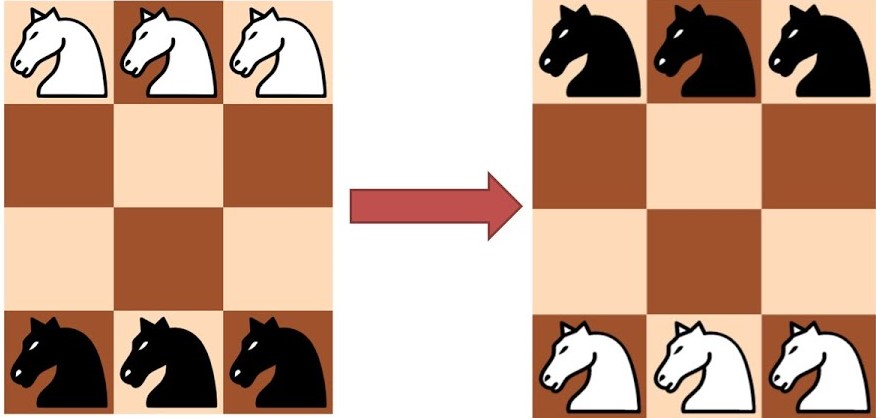
\includegraphics[width=70mm]{guarini}
    \caption{Puzzle-ul lui Guarini}
    \label{fig:method}
    \end{figure}
    
\section{Modelarea Problemei}
    Pentru modelarea problemei, vom reține starea tablei într-o matrice de caractere, caracterul W și B pentru caii de culoare albă, respectiv, neagră și caracterul "\_" pentru spațiu gol:
    
    Stare inițială: Si = 
    $\begin{bmatrix} 
    W & W & W\\
    \_ & \_ & \_\\
    \_ & \_ & \_\\
    B & B & B
    \end{bmatrix}$
    
    Stare finală: Sf = 
    $\begin{bmatrix} 
    B & B & B\\
    \_ & \_ & \_\\
    \_ & \_ & \_\\
    W & W & W
    \end{bmatrix}$
    
    Starea generală este de forma: S =
    $\begin{bmatrix} 
    X00 & X01 & X02\\
    X10 & X11 & X12\\
    X20 & X21 & X22\\
    X31 & X32 & X33
    \end{bmatrix}$
    
    Unde Xij $\in$ \{W, B, \_ \} 
    Pentru dificultatea ușoară: $i=\overline{0,3}$, $j=\overline{0,2}$
    
    \hfill \break
    Pentru dificultățile mediu și greu, numărul de coloane este incrementat.
    \hfill \break
    Operatorii pentru modificarea stării pieselor sunt de forma: 
    \\((X-piesă, Y-piesă),(X-offset, Y-offset))
    \\Unde valorile valide pentru offset sunt toate combinațiile (x, y) de forma: $(\pm1, \pm2) sau (\pm2, \pm1)$  

\section{Implementare}
    Algoritmii folosiți in rezolvarea problemei lui Guarini sunt următorii: \hfill \break
    -Depth first search \hfill \break
    -Breadth first search \hfill \break
    -uniform cost \hfill \break
    -A* cu euristicile: \begin{itemize}
                                        \item easy care numără câte piese nu au ajuns pe pozitia finală
                                        \item cea care estimează distanța până la rândul destinație și pe aceeași coloană a piesei
                                        \item cea care estimează
                         distanța până la pozițiile libere de pe rândul destinație   \end{itemize}
           
    Toți algoritmii utilizează conceptele de frontieră și teritoriu pentru căutarea în spațiu stărilor. Teritoriul reprezintă stările deja explorate, iar în frontieră sunt reținute stările neexplorate și adiacente stărilor din teritoriu. 
    
    Pentru a găsi stările succesor pentru o configurație a tablei se utilizează funcția expand(). Aceasta execută toți operatorii aplicabili asupra tablei și returnează toate stările succesor găsite alături de operatorul respectiv.
    
    
   \textbf{ Depth first search} \hfill \break  
        Acest algoritm expandează starea curentă și adaugă în stiva folosită ca frontieră stările găsite. Această implementare explorează cât mai mult de-a lungul unei ramuri, în ”adâncime” înainte de a explora ramuri adiacente. După mai multe rulări, s-a observat că acest algoritm de căutare nu este potrivit pentru problema lui Guarini, deoarece găsește cea mai ineficientă cale posibilă.
        \hfill \break
        Pentru a optimiza algoritmul, teritoriul este reținut într-o structură de date de tip set cu scopul de a verifica dacă o stare se află deja în teritoriu în timp O(1). Frontiera utilizează în același timp o stivă (pentru procesarea stărilor în ordinea LAST IN-FIRST OUT) și un set (pentru verificarea existenței unei stări din frontieră mai rapidă).
        
        
    \textbf{Breadth first search}\hfill \break
        Acest algoritm explorează spațiul stărilor în ”lățime”, explorând întotdeauna complet un nivel al ramificațiilor, înainte de a coborî la următorul nivel. Astfel, procesarea unei stări constă în expandare și adăugarea în coada de așteptare (frontieră) a starilor succesor. Algoritmul este potrivit pentru căutări unde factorul de ramificație este mic, iar soluția se află la o adâncime relativ mică.\hfill \break
        Pentru a optimiza algoritmul, teritoriul este reținut într-o structură de date de tip set cu scopul de a verifica dacă o stare se află deja în teritoriu în timp O(1). Frontiera utilizează în același timp o coadă (pentru procesarea stărilor în ordinea FIRST IN-FIRST OUT) și un set (pentru căutarea stărilor din frontieră mai rapidă).

            
    \textbf{Uniform cost search}\hfill \break
        Acest algoritm explorează spațiul stărilor în funcție de costul căii curente ( reia explorarea stărilor care au asociat costul cel mai mic ). Deoarece în cazul acestui puzzle toate mutările au cost 1, costul reprezintă lungimea sau numărul de mutări necesare de a ajunge din starea inițială în starea următoare. Algoritmul de cost uniform, în cazul în care toate tranzițiile au costuri egale, se comportă la fel ca algoritmul de căutare în lățime, Breadth first search.
        Cu toate acestea, timpul de execuție al acestei implementări este mai mare din cauza overhead-ului utilizării cozii de priorități.

     \textbf{A* search}\hfill \break
        Acest algoritm explorează spațiul stărilor în funcție de costul căii curente și funcția euristică utilizată. Se pornește de la ideea algoritmului de cost uniform, dar se adaugă una din cele 3 funcții euristice care estimează un cost mai mic pentru stările apropiate de starea finală.\hfill \break Avem 3 euristici:
        \begin{itemize}
        
        \item Euristica care numără câte piese nu sunt pe poziția finală: astfel stările ce au mai multe piese pe poziția finală vor avea un cost mai mic și vor fi alese mai repede.\hfill \break
        Pentru celelalte 2 euristici, ne folosim de o matrice precalculată ce conține numărul de mutări până la fiecare poziție, din orice poziție s-ar afla piesa, accesând din matrice cu offset-urile de deplasare.\hfill \break
        
    $MatriceDeAproximare=\begin{bmatrix} 
    0 & 3 & 2 & 5 & 2\\
    3 & 4 & 1 & 2 & 3\\
    2 & 1 & 4 & 3 & 2\\
    5 & 2 & 3 & 2 & 3\\
    \end{bmatrix}$\hfill \break
        Exemplu: pentru a afla de câte mutări este nevoie să mutăm o piesă din orice poziție la o distanță de 3 rânduri și 2 coloane, accesăm din matrice elementul [3][2] care este = 3.
        
        \item
        Euristica de aproximare a distanței până la rândul destinație și pe aceeași coloană a piesei.Pentru această euristică, se face suma mutărilor tuturor pieselor până la rândul destinație.
        \item Euristica de aproximare a distanței până la pozițiile libere de pe rândul destinație.Pentru fiecare piesă se verifică dacă este pe poziție finală și in funcție de asta se decrementează euristica (stările care au cost mai mic sunt explorate mai repede), altfel se calculează media distanței până la pozițiile neocupate (de piese de aceeasi culoare). 
        
        \end{itemize}
        
\section{Comparare algoritmi}

\textbf{Noduri expandate}
\begin{center}
\begin{tabular}{||c c c c||} 
 \hline
  & dificultate 1 & dificultate 2 & dificultate 3 \\ [0.5ex] 
 \hline\hline
 dfs & 14437 & notDef & notDef \\ 
 \hline
 bfs & 17175 & 898770 & notDef \\
 \hline
 cost uniform & 17175 & 898770 & notDef \\
 \hline
 A* easy & 1615 & 117 & 227 \\
 \hline
 A* same column & 162 & 47 & 29 \\ 
  \hline
 A* average & 252 & 177 & 104 \\ [1ex] 
 \hline
\end{tabular}
\end{center}

\hfill \break
\textbf{Cost}
\begin{center}
\begin{tabular}{||c c c c||} 
 \hline
  & dificultate 1 & dificultate 2 & dificultate 3 \\ [0.5ex] 
 \hline\hline
 dfs & 984 & notDef & notDef \\ 
 \hline
 bfs & 16 & 16 & notDef \\
 \hline
 cost uniform & 16 & 16 & notDef \\
 \hline
 A* easy & 16 & 18 & 22 \\
 \hline
 A* same column & 18 & 18 & 22 \\ 
  \hline
 A* average & 18 & 20 & 22 \\ [1ex] 
 \hline
\end{tabular}
\end{center}


\hfill \break
\textbf{Timp rulare (sec)}
\begin{center}
\begin{tabular}{||c c c c||} 
 \hline
  & dificultate 1 & dificultate 2 & dificultate 3 \\ [0.5ex] 
 \hline\hline
 dfs & 5.5 & notDef & notDef \\ 
 \hline
 bfs & 4.8 & 484.3 & notDef \\
 \hline
 cost uniform & 100.8 & $>$ 10 ore & notDef \\
 \hline
 A* easy & 3.6 & 0.19 & 2.38 \\
 \hline
 A* same column & 0.06 & 0.13 & 0.07 \\ 
  \hline
 A* average & 0.21 & 0.51 & 0.6 \\ [1ex] 
 \hline
\end{tabular}
\end{center}
În cazul valorilor notDef, algoritmii nu au putut fi rulați din cauza constrângerilor de timp și resurse ale calculatorului(dfs dificultate 2 a utilizat complet memoria RAM a calculatorului, teritoriul ajungând la dimensiunea de 200 000, iar bfs dificultate 3 a rulat timp de 6 ore, frontiera ajungând la 4 000 000).

Comparând algoritmii fără euristică, se observă faptul că bfs si cost uniform sunt mai potriviți pentru această problemă, deoarece soluția se află la o adâncime relativ mică: 16 pași. Deși bfs și cost uniform expandează mai multe stări, aceștia găsesc soluția optimă, iar dfs găsește o soluție extrem de inefiecientă cu 984 de pași. Timpul de execuție mărit de la algoritmul de cost uniform se datorează duratei mare de inserare și căutare în structura ”coadă de priorități”. Cea mai mare eficiență dintre cei 3 algoritmi o are bfs, acesta fiind executat cu succes și pentru dificultatea medie.
    Doar bfs și cost uniform sunt optimali, deoarece aceștia găsesc prima dată cea mai eficientă soluție. Dfs nu este optimal.
    Pentru dificultatea medie, numai algoritmul bfs a fost executat cu succes, acesta găsind o soluție cu 16 pași și cu un număr de 898770 noduri expandate.
    
    
Algoritmul A* este mult mai rapid și eficient decât algoritmii fără euristici (din punct de vedere al nodurilor expandate și a timpului de execuție), dar nu găsește întotdeauna cea mai eficientă cale. Toate cele trei euristici reușesc să găsească soluții pentru cele 3 dificultăți într-un timp scurt și număr mic de noduri expandate. În ceea ce privește numărul de noduri expandate, euristica cu cele mai puține expandări pentru toate dificultățile este euristica de aproximare pe aceeași coloană. Din punct de vedere al costului, easy heuristic este singura care găsește soluția optimă pentru dificultatea 1.

\end{document}
